\chapter{Implementing the Complete \lambdacalculus}

The \lambdacalculus{} is a formal system developed by Church in the 1930's to
study the computational aspects of functions~[13]. It is a relatively simple
system, consisting of a small syntax for constructing terms and three rewrite
rules for transforming terms. Although it is simple, the \lambdacalculus{} is an
extremely powerful system, capable of describing all computable functions.

This chapter presents Church's pure, untyped \lambdacalculus{} and some of the
issues and problems regarding its efficient implementation. Previous attempts to
deal with these issues are recounted, and an alternate interpretation of the
operational \lambdacalculus{} based on Berkling's head order reduction
theory~[11] is offered as a viable solution to these problems.

\section{The Pure Untyped \lambdacalculus}

\subsection{Syntax}

The abstract syntax of the pure, untyped \lambdacalculus{} (hereafter simply
referred to as the pure \lambdacalculus) defines the set of allowable
\(\lambda\)-expressions as
\[
\begin{aligned}
x &\in \textit{Identifiers}\\
e &\in \lambda\textit{-Expressions}\\
e &::= x \mid \lambda x.e \mid e_1 e_2 .
\end{aligned}
\]

Expressions of the form \(\lambda x.e\) are called \emph{abstractions}.
Abstractions represent the notion of functions in the \lambdacalculus. The
identifier \(x\) is referred to as the abstraction's \emph{bound variable},
which acts as a formal parameter for the function. The subexpression \(e\) is
the \emph{body} of the abstraction.

Expressions of the form \(e_1 e_2\) are called \emph{applications}.
Applications represent the application of a function, \(e_1\), to an argument,
\(e_2\). By convention, application is left associative; this can be
circumvented through the use of parentheses.

When no confusion will arise, the bound variables of multiple abstractions will
often be written between a single \(\lambda\) and dot. For example, the
expression \((\lambda x.\lambda y.e)\) can also be written as
\((\lambda xy.e)\).

\subsection{Semantics}

Before presenting the rewrite rules of the pure \lambdacalculus, two
definitions are necessary:

\begin{definition}[Free Variable]
The free variables of an expression \(e\) are defined by the following rules:
\[
\begin{array}{rcl}
1. & \fv(x) &= \{x\}\\
2. & \fv(e_1e_2) &= \fv(e_1) \cup \fv(e_2)\\
3. & \fv(\lambda x.e) &= \fv(e) - \{x\}.
\end{array}
\]
An occurrence of the variable \(x\) in the expression \(e\) is free with respect
to \(e\) if and only if \(x \in \fv(e)\). If an expression \(e\) has no free
variables, i.e. \(\fv(e)=\{\}\), \(e\) is said to be \emph{closed}.
\end{definition}

\begin{definition}[Substitution]
The substitution of an expression \(e_1\) for all free occurrences of an
identifier \(x\) in an expression \(e_2\) is written as \([e_1/x]e_2\) and is
defined by the following rules:
\[
\begin{array}{rcll}
1. & [e_1/x]x &= e_1\\
2. & [e_1/x]y &= y, & \text{where } x \ne y\\
3. & [e_1/x](e_2e_3) &= ([e_1/x]e_2\ [e_1/x]e_3)\\
4. & [e_1/x](\lambda x.e_2) &= \lambda x.e_2\\
5. & [e_1/x](\lambda y.e_2) &= \lambda y.[e_1/x]e_2,\\
\end{array}
\]
if \(x \ne y\) and either \(y \notin \fv(e_1)\) or \(x \notin \fv(e_2)\);
\[
6.\quad [e_1/x](\lambda y.e_2)=\lambda z.[e_1/x]([z/y]e_2),
\]
if \(x \ne y\), \(y \in \fv(e_1)\), \(x \in \fv(e_2)\), and
\(z \notin \fv(e_1) \cup \fv(e_2)\).
\end{definition}

The last rule in the definition of substitution handles the case where a name
conflict occurs and is resolved by a name change. This situation is quite
subtle, and expensive to detect and correct.

There are three rewrite rules defined on \(\lambda\)-expressions:

\begin{enumerate}
\item \(\alpha\)-conversion:
  \(\lambda x.e \longleftrightarrow \lambda y.[y/x]e\), where \(y \notin \fv(e)\).
\item \(\beta\)-conversion:
  \((\lambda x.e_1)e_2 \longleftrightarrow [e_2/x]e_1\).
\item \(\eta\)-conversion:
  \(\lambda x.(e\ x) \longleftrightarrow e\), if \(x \notin \fv(e)\).
\end{enumerate}

The reflexive, transitive closure of these rules forms a theory of
convertibility on the \lambdacalculus{} that is consistent as a mathematical
system.

The \lambdacalculus{} as defined by the rewrite rules above is what Hindley and
Seldin~[25] refer to as the \(\lambda\beta\eta\)-calculus. This dissertation is
only concerned with implementing the \lambdabetacalculus, which is composed of
only the first two rules. Furthermore, \(\beta\)-conversion will be restricted
so that conversion can only happen in one direction:
\[
\beta\text{-Reduction:}\quad (\lambda x.e_1)e_2 \longrightarrow [e_2/x]e_1 .
\]
The notation \(\longrightarrow\) will be used to denote the reflexive,
transitive closure of \(\longrightarrow\) including \(\alpha\)-conversions, and
\(\longrightarrow^n\) will denote \(n\) applications of the
\(\beta\)-reduction rule with possible \(\alpha\)-conversions.

\subsection{Normal Form}

Expressions in the \lambdabetacalculus{} are transformed through application of
the \(\beta\)-reduction rule. An occurrence of the left hand side of a rewrite
rule is called a \emph{redex}, which may be replaced by the right hand side of
the rule, called the \emph{contractum}. The replacement of a redex by its
contractum is referred to as a \emph{reduction} or \emph{contraction}. These
concepts lead to the following notion:

\begin{definition}[Normal Form]
A \(\lambda\)-expression is in \emph{normal form} if it cannot be further
transformed using the \(\beta\)-reduction rule.
\end{definition}

It should be noted that not all \(\lambda\)-expressions have a normal form. For
example, the expression
\[
(\lambda x.(x\ x))(\lambda x.(x\ x))
\]
reduces to itself.

Because they contain no more redexes, normal forms are often considered to
canonically represent the ``value'' of \(\lambda\)-expressions. This view is
justified by Church-Rosser Theorem I~[50], which states that if a normal form
for an expression exists, that normal form is unique up to \(\alpha\)-conversion.

A consequence of this theorem is that how a normal form is generated is not
important; that is, the order in which redexes are contracted is irrelevant.
This raises an important question: if a normal form exists, is it always
possible to find it? The answer is provided by Church-Rosser Theorem II, which
states that if a normal form \(e'\) exists for an expression \(e\), then there
exists a normal order reduction sequence from \(e\) to \(e'\).

\begin{definition}[Normal Order Reduction]
A normal order reduction is a sequence of reductions such that whenever there is
more than one redex in an expression, the leftmost redex is always selected for
contraction.
\end{definition}

While the choice of which redex to contract may make no difference in theory, in
practice it has a strong impact on the behavior and efficiency of
\lambdacalculus{} implementations. This point will be taken up again in the
Section 2.2.3.

\section{Implementation Issues}

Although the \lambdacalculus{} as presented above may seem simple, it has proven
notoriously difficult to implement efficiently and correctly. This section
presents some of the reasons why this is so, how others have dealt with these
problems, and how RED2 deals with them.

\subsection{Representation of Expressions}

One of the most important characteristics of the \lambdacalculus{} that is often
ignored by implementors is that the rewrite rules of the \lambdacalculus{}
transform \emph{expressions into expressions}. A complete implementation of the
\lambdacalculus{} should accept expressions as input and produce expressions as
output. For example, the input expression
\[
(\lambda x.\lambda y.(+\,y\,(*\,x\,4)))\ 2
\]
should produce the output expression
\[
(\lambda y.(+\,y\,8)).
\]

(The execution of procedures without applying all the necessary arguments is
generally referred to as partial evaluation.) This may seem obvious to even the
casual observer, but the implications are far reaching and constrain one's
choice of ``program'' representation.

To fully implement the \lambdacalculus, then, a computing system must retain
information about the changing structure of expressions, so that they can be
re-created upon output. This constrains the possible machine representations of
expressions; two representations that have been extensively studied are strings
and graphs. Previous work with the RED1 reduction machine~[32] has shown that
strings are not viable as an efficient vehicle for sequential computation.
\footnote{Mago~[38] has proposed a massively parallel string reduction machine
for Backus' FP language~[7], but no hardware implementation has yet been built.}
In RED2, \(\lambda\)-expressions are represented as directed graphs.

The notion that the result of executing a piece of software should result in
another piece of software is a radical one to most computer scientists.
\footnote{I am speaking at the programming language level, not about programs
themselves. There are plenty of programs that manipulate other programs; there
is nothing radical about this kind of ``meta'' manipulation. In the
\lambdacalculus, however, programs transform themselves into other (equivalent)
programs via reduction - there is nothing ``meta'' going on here.} Almost all
conventional programming language implementations in widespread use (including
functional languages based on the \lambdacalculus) take a procedure or
expression as input and produce one or more ``values'' as output, where the
values are restricted to grounded data objects.\footnote{Logic programming
languages are an exception in that they allow ungrounded data objects to be
produced as a result of computation. Some experimental logic languages, such as
SUPER~[49], also allow logic expressions (such as disjunctions of clauses) to be
produced as output; however, none of the widely available logic programming
languages that I am aware of allows this.} Consequently, there is no need to
preserve the syntactic structure of procedures at run-time. (Certain compilers
and systems do preserve program structure, but this is done for debugging
purposes, not because the structure is part of the computation result.)

I believe this view of computation as ``producing values'' is a historic
artifact of the von-Neumann computing architecture, which has dominated the
thinking of computer scientists. This view is not necessarily wrong; it has
become the predominant view precisely because it is appropriate to almost all of
the computational tasks currently done. However, this view is limiting; it denies
most people the chance to understand, appreciate, and utilize a more general
concept of computation.

\subsection{Incremental Reduction}

The ``value producing'' view of computation also explains why the concept of
normal form is so appealing to language implementors. An expression in normal
form is ``computationally complete'' in the sense that no more redexes can be
contracted, and therefore reflects the ``value'' of an expression. The desire to
produce a value is so strong that even functional languages are designed and
implemented so as to keep reducing until a normal form is produced.

This desire is solely human in origin; there is no ``force'' within the
\lambdacalculus{} that drives expressions to their normal form. There is no
fundamental reason that an implementation of \lambdacalculus{} should insist on
reducing to normal form. Indeed, in certain contexts non-normal form expressions
might be of interest. Therefore, the RED2 architecture allows the user to
incrementally reduce expressions by specifying the maximum number of reductions
that may be performed on an expression (as did RED1).

Incremental reduction has a strong effect on the semantics and implementation
of many features of THOR, the reduction language directly executed by RED2. In
theory, each reduction in functional languages is semantically an atomic event;
in practice, however, many implementations take advantage of the fact that
reduction continues until a normal form is reached to interleave many reductions
in order to achieve higher performance (see the discussion in Section 2.2.4 on
substitution). Designing THOR so that incremental reduction is both efficient and
semantically consistent presented some interesting challenges which will be
discussed in more detail in Chapter 3.

Incremental reduction also has the pleasant side-effect that non-terminating
reduction sequences are not allowed to go unchecked. Eventually the number of
allowed reductions is exhausted, and reduction stops.

\subsection{Order of Reduction}

According to Church-Rosser Theorem I, the order in which redexes in an
expression are chosen for contraction is irrelevant to producing the expression's
normal form, if one exists. In practice, however, the order of reduction has a
direct bearing on the efficiency and behavior of any \lambdacalculus{}
implementation. Take, for example, the following normal order reduction
sequence, where the redex to be contracted is underlined:
\[
\begin{aligned}
(\lambda x.\lambda y.y\ x\ x)(\lambda z.((\lambda w.w)\ z))
&\longrightarrow\\
(\lambda y.y\ (\lambda z.((\lambda w.w)\ z))\ (\lambda z.((\lambda w.w)\ z)))
&\longrightarrow\\
(\lambda y.y\ (\lambda z.z)\ (\lambda z.((\lambda w.w)\ z)))
&\longrightarrow\\
(\lambda y.y\ (\lambda z.z)\ (\lambda z.z)).
\end{aligned}
\]
This sequence takes three reductions. Notice that each copy of the substituted
argument is reduced separately. However, if the order of redex contraction is
changed, the argument need only be reduced once:
\[
\begin{aligned}
(\lambda x.\lambda y.y\ x\ x)(\lambda z.((\lambda w.w)\ z))
&\longrightarrow\\
(\lambda x.\lambda y.y\ x\ x)(\lambda z.z)
&\longrightarrow\\
(\lambda y.y\ (\lambda z.z)\ (\lambda z.z)).
\end{aligned}
\]
The strategy of reducing arguments before they are applied is called
applicative order reduction.

Although applicative order reduction often saves work, it does not always
produce a normal form when one exists. For example, the expression
\[
(\lambda x.\lambda y.y)((\lambda x.x\ x)(\lambda x.x\ x))
\]
correctly reduces to \((\lambda y.y)\) using normal order reduction, but fails
to converge under a sequential applicative order reduction.

There have been other reduction strategies published in the literature, some of
which are more efficient than normal order reduction~[34]. However, because
normal order reduction is simple to implement and always produces a normal form
when one exists, it was chosen as the reduction strategy for RED2. It will later
be shown how to regain much of the savings of applicative order reduction by
sharing the results of some subgraph reductions.

\subsection{Substitution}

Substitution is the most basic operation in the \lambdacalculus, and it is also
the most expensive. The cost can be broken down into two parts: the act of
replacing a variable's free occurrences in the body of a contracted
\(\beta\)-redex, and the check for and correction of name clashes. Different
strategies have been developed to try and minimize the cost of substitution.

\subsubsection*{Delaying Substitution}

A naive reading of the \(\beta\)-reduction rule says that upon contraction,
every occurrence of the bound variable in the body is replaced by the argument
all at once. This is a correct but very expensive interpretation of the
\(\beta\) rule, because each time a \(\beta\)-reduction occurs, a new copy copy
of the body is created. For example, consider the abstraction
\[
\lambda a.\lambda b.\lambda c.e
\]
When this abstraction is fully applied, the body of the abstraction would be
copied three times - once for each bound variable in its scope.

A more efficient method is to delay argument substitution as long as possible,
and then substitute all of the arguments at once. Then only one copy of the body
need be made. This is the basic idea underlying Landin's SECD machine~[33]. Two
new concepts are necessary to delay substitution: the environment and the
closure. An environment is a mapping from variables to values, and is
traditionally written as \(\rho\). A closure is an expression \(e\), and an
environment \(\rho\) of delayed substitutions that are to be applied to \(e\),
and will be written as \(e\{\rho\}\). Using these new ideas, the
reduction/substitution process can be redefined:
\[
\begin{array}{rcl}
1. & x\{\rho\} &= \rho(x)\\
2. & (e_1e_2)\{\rho\} &= (e_1\{\rho\}\ e_2\{\rho\})\\
3. & (\lambda x.e)\{\rho\} &= \lambda x.(e\{\rho + [x/x]\})\\
4. & (\lambda x.e_1\{\rho_1\})e_2\{\rho_2\}
   &= e_1\{\rho_1 + [e_2\{\rho_2\}/x]\}.
\end{array}
\]
Note that each \(\beta\)-reduction is now composed of many incremental steps
instead of being one monolithic action.

The equations above can be implemented in many different ways. Landin did not
try to manipulate a direct representation of \(\lambda\)-expressions; instead he
designed a fixed-program machine with four registers: the Stack, Environment,
Control, and Dump (hence the name SECD).\footnote{This machine was refined and
popularized by Henderson~[24].}

One should also note that delaying substitution by itself does nothing about
avoiding name clashes. Some common solutions to this problem are:

\begin{enumerate}
\item Always perform \(\alpha\)-conversion on the abstraction before performing
\(\beta\)-reduction, while insuring that the renamed variable is unique. This
solution can hardly be considered efficient, since it requires that each
\(\beta\)-reduction be accomplished by two substitutions - one for the renamed
variable and the other for the argument.
\item Do away with variable names, replacing them with something that depends
only on an expression's structure. DeBruijn indices~[12], which represent bound
variables by indicating the number of lambda bindings appearing between the
variable and its binding occurrence, have proven effective in this role.
\item Prevent name clashes by forbidding the reduction of abstractions that are
not applied to arguments. This solution, which clearly violates the semantics of
the pure \lambdacalculus, is the one adopted by most functional language
implementors.
\end{enumerate}

\begin{figure}
\centering
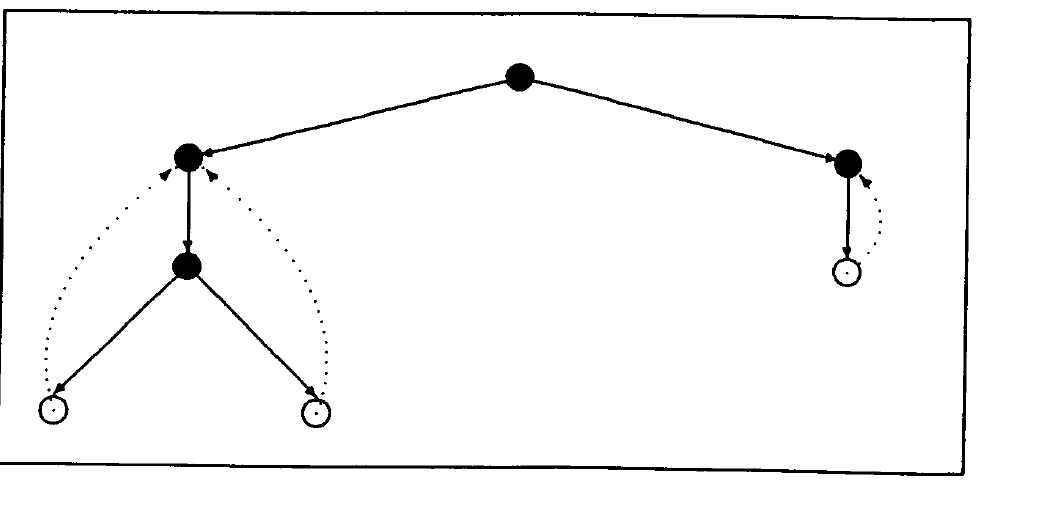
\includegraphics[width=0.75\textwidth]{assets/figure-2-1.png}
\caption{The expression \(((\lambda x.xx)(\lambda y.y))\) represented in
Wadsworth's graph notation. The filled circles with two outgoing arcs are
application nodes; those with one outgoing arc are abstractions. The hollow
circles are variables. The dotted lines are backpointers from variables to their
bindings.}
\end{figure}

\subsubsection*{Graph Reduction}

At the other end of the substitution spectrum is \emph{graph reduction},
developed by Wadsworth~[61]. Unlike Landin's environment, which communicates
argument values to each free variable separately as needed, Wadsworth's graphs
make each substitution a single event which communicates the argument value to
every free occurrence of a bound variable simultaneously.

Expressions are represented as ordered, directed acyclic graphs. Applications
are represented by a graph node with two outgoing arcs, one of which points to
the application's operator and the other points to the operand. Abstractions are
represented by nodes with a single outgoing arc, which points to the graph
representing the body of the abstraction. Free occurrences of the abstraction's
bound variable are represented by leaf nodes which contain a special kind of arc
that points back to the root node of the abstraction. Figure 2.1 shows an
example of this representation.

In Wadsworth's system, \(\beta\)-reduction is performed by manipulating pointers
rather than by direct substitution. When a \(\beta\)-redex is contracted, two
things happen: the abstraction node is ``overwritten'' by an indirection arc
which points to the argument, and the root node of the redex is overwritten by
an indirection arc which points to the abstraction's body. (See Figure 2.2.)
These two actions are all that is necessary for each free variable occurrence to
``feel'' the effects of substitution. And since each bound variable is
represented by a unique node in the graph, the name clash problem disappears.

The simple version of graph reduction presented above does not suffice for all
situations. In the case when an abstraction is the operator of a
\(\beta\)-redex and is pointed to by more than one application node, the
portions of the abstraction's body which contain references to the abstraction's
bound variable must be copied before contraction can take place, or erroneous
results may occur.

Detecting such a situation is expensive, for it entails checking every
application node in the graph to see if more than one points to the abstraction
in question every time a \(\beta\)-redex is contracted! Alternatively, some sort
of reference counting scheme could be devised to alleviate the checking of
application nodes. Aiello and Prini~[2] conclude that, rather than perform such
a check every reduction, it is cheaper to always copy the abstraction before
contraction occurs. The cost of each of these remedies is prohibitive, and this
style of graph reduction has never become popular.

\begin{figure}
\centering
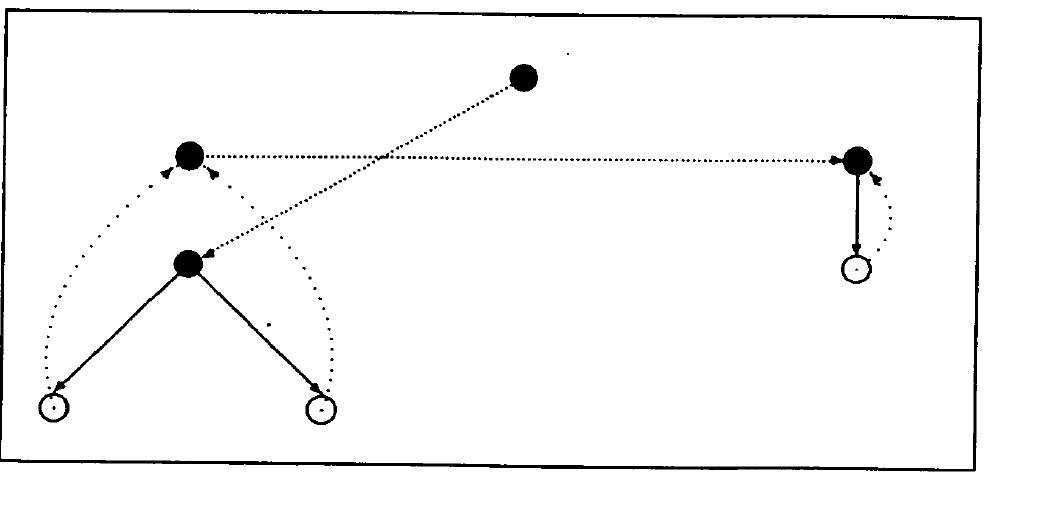
\includegraphics[width=0.75\textwidth]{assets/figure-2-2.png}
\caption{The graph after contraction of the \(\beta\)-redex. The dashed arcs
represent indirection pointers.}
\end{figure}

\subsubsection*{Eliminating Substitution}

Perhaps the most radical solutions proposed are those that eliminate
substitution altogether! This can be accomplished in two basic ways, by either
eliminating variables from expressions or by reformulating the rewrite rules of
the \lambdacalculus{} so as to avoid substitution.

Combinators are the best known solution of the first type. Schonfinkel~[53]
showed that it is possible to do away with variables altogether with the use of
three special constants, \(S\), \(K\), and \(I\), called combinators, which have
the following rewrite rules:
\[
\begin{aligned}
S\ f\ g\ x &\longrightarrow ((f\ x)(g\ x))\\
K\ x\ y &\longrightarrow x\\
I\ x &\longrightarrow x
\end{aligned}
\]
Using these three combinators, any expression containing bound variables can be
transformed into an equivalent bound-variable free expression.

Turner~[60] introduced the use of combinators for implementing functional
languages in the late 1970's. The SKI-calculus and its relatives give rise to
very simple reduction machines which only have to support a fixed set of
combinators and need no argument substitution mechanism. As a result,
combinator reducers are easy to build, and when they were first introduced they
out-performed other types of \(\lambda\)-reducers by about three to one~[43].
This new found speed and simplicity touched off a flurry of interest in
combinators, which resulted in two specialized hardware implementations:
SKIM~[59], developed at Cambridge, and NORMA~[52], developed by the Burroughs
Corporation. More efficient \(\lambda\)-reducers have since been developed,
making combinators less attractive as an implementation strategy. With the
exception of a few researchers~[42], combinators have fallen out of general use.

Solutions of the second type have not yet made a great impact on
\(\lambda\)-calculus implementations, but have potential for doing so.
Revesz~[47] presents a redefinition of the \(\beta\)-reduction rule which does
away with explicit substitution and avoids name conflicts. His new system was
formulated with parallel reduction in mind. Berkling presents another such
system, the theory of head order reduction, which forms the basis of my
implementation work.

\section{The Theory of Head Order Reduction}

In~[11], Berkling presents a new formulation of the operational
\lambdacalculus, the theory of head order reduction. Head order reduction was
developed expressly to provide a basis for efficient, complete implementations
of the \lambdacalculus. A proof that head order reduction is a sound and
complete formulation of the \lambdacalculus{} is provided by Zhang~[62].

Before presenting head order reduction, the following definition is needed:

\begin{definition}[Head Normal Form]
A \(\lambda\)-expression is said to be in \emph{head normal form} if it is of
the form
\[
(\lambda x_1\cdots x_m.x_i e_0\cdots e_n)
\]
where \(1 \le i \le m\). In other words, the \emph{head} of the expression is a
variable and is not a redex of any kind.
\end{definition}

Head order reduction consists of three rewrite rules:

\begin{enumerate}
\item \(\underline{\eta_{ext}}\) (Eta-extension in-the-large):
\[
(\lambda y_1\cdots y_m.e_0)e_1\cdots e_n
\longrightarrow
\lambda z_1\cdots z_{m-n}.((\lambda y_1\cdots y_m.e_0)e_1\cdots e_n
z_{m-n}\cdots z_1)
\]
where \(m > n\) and each \(z_i \notin \fv(e_0)\cup\cdots\cup\fv(e_n)\).

\item \(\underline{\beta_{ext}}\) (Beta-extension in-the-large):
\[
(\lambda y_1\cdots y_m.e_0\cdots e_k)E_1\cdots E_n
\longrightarrow
e'_0\cdots e'_k E_{m+1}\cdots E_n
\]
where \(m \le n\) and
\[
e'_i=((\lambda y_1\cdots y_m.e_i)E_1\cdots E_m).
\]

\item \(\underline{\beta_h}\) (Identity-reduction in-the-large):
\[
(\lambda y_1\cdots y_m.y_i)e_1\cdots e_m \longrightarrow e_i
\]
where \(1 \le i \le m\).
\end{enumerate}

Head order reduction attempts to delay \(\beta\)-reduction as long as possible
by repeatedly ``pushing'' copies of \(\beta\)-redexes through application nodes
until they are piled up in front of variables. This pushing is accomplished by
the cooperative effort of the \(\eta_{ext}\) and \(\beta_{ext}\) rules: the
\(\eta_{ext}\) rule makes certain there are an equal number of bindings and
arguments to be pushed, and the \(\beta_{ext}\) rule does the actual pushing.
When the \(\beta\)-redexes have been pushed all the way down to the variables,
the head of the expression is in the form of a \(\beta_h\)-redex. When this
redex is contracted, one of the \(e_i\) is selected (the rest of the redex
disappears). These rules are repeatedly applied until every subexpression is in
head normal form, thereby signaling the entire expression is in normal form.

It is important to note the following:

\begin{itemize}
\item Nowhere in these rules is substitution mentioned. Substitution is not a
part of head order reduction.
\item Every \(\lambda\)-expression is either in normal form or contains at
least one subexpression which matches one and only one of the three redexes
presented above (Zhang, Lemma 1).
\item If each of the \(z_i\) introduced by contractions of the \(\eta_{ext}\)
rule is unique, then there will be no name clashes. This follows from the
observation that every bound variable remaining in an expression's normal form
is generated by an application of \(\eta_{ext}\).
\end{itemize}

The shrewd observer may have noticed that although substitution has been
eliminated, head order reduction does not necessarily make it any easier to
reduce \(\lambda\)-expressions. In fact, head order reduction seems to be
\emph{more difficult}! Copying and pushing all those redexes around takes a lot
of time and space.

Much work can be avoided if only a single copy of the pushed redexes is kept in
a read-only structure called the \emph{redex store}, which preserves the correct
redex ordering. Because the redex store is read-only, it may be freely shared;
pointers into the appropriate place in the redex store may now be propagated by
the reduction rules instead of the actual redexes themselves. The redex store is
analogous to the environment introduced in Section 2.2.4; so much so, that the
same notation will be used for both. The head order reduction rules can now be
rewritten to use the redex store \(\rho\):

\begin{enumerate}
\item \(\underline{\eta'_{ext}}\):
\[
((\lambda y_1\cdots y_m.e_0)e_1\cdots e_n)\{\rho\}
\longrightarrow
(\lambda z_1\cdots z_{m-n}.(e_0\{\rho'\}))
\]
where \(m > n\),
\[
\rho'=\rho+[e_1\{\rho\}/y_1,\ldots,e_n\{\rho\}/y_n,
z_{m-n}/y_{n+1},\ldots,z_1/y_m],
\]
and each \(z_i \notin \fv(e_0)\cup\cdots\cup\fv(e_n)\).

\item \(\underline{\beta'_{ext}}\):
\[
((\lambda y_1\cdots y_m.e_0\cdots e_k)E_1\cdots E_n)\{\rho\}
\longrightarrow
e_0\{\rho'\}\cdots e_k\{\rho'\}E_{m+1}\{\rho\}\cdots E_n\{\rho\}
\]
where \(m \le n\) and
\[
\rho'=\rho+[E_1\{\rho\}/y_1,\ldots,E_m\{\rho\}/y_m].
\]

\item \(\underline{\beta'_h}\): \(y\{\rho\}\longrightarrow \rho(y)\).
\end{enumerate}

Note that the \(\eta_{ext}\) rule has now incorporated the knowledge that a
\(\beta_{ext}\) reduction would normally be accomplished next, and so performs
both in one step.

\section{Deriving an Architecture}

The rules presented in the previous section are concerned with simultaneously
manipulating arbitrarily large portions of an expression, hence the descriptor
``in-the-large.'' These rules are a suitable basis for directly implementing a
concurrent or parallel reduction system. The development of such a system is an
eventual goal of the RED project. For the initial head order reduction-based
machine, however, a single processor sequential system was chosen as a testbed
for different implementation ideas and as a proof-of-concept demonstration. The
in-the-large rules are not very suitable for implementation by a simple
sequential automaton; a more appropriate set of rules are these equivalent
``in-the-small'' rules:

\begin{enumerate}
\item \(\underline{\beta''_{ext}}\):
\[
((\lambda y.e_0)e_1)\{\rho\}\longrightarrow e_0\{\rho+[e_1\{\rho\}/y]\}
\]
\item \(\underline{\Omega}\):
\[
(e_0e_1)\{\rho\}\longrightarrow ((e_0\{\rho\})(e_1\{\rho\}))
\]
\item \(\underline{\eta''_{ext}}\):
\[
(\lambda y.e)\{\rho\}\longrightarrow \lambda z.(e\{\rho+[z/y]\}),
\quad \text{where } z\notin \fv(e).
\]
\item \(\underline{\beta''_h}\): \(y\{\rho\}\longrightarrow \rho(y)\).
\end{enumerate}

Notice that a new rule has been introduced and the rule ordering has been
changed. Both of these changes are significant.

The \(\Omega\) rule is necessary because \(\beta''_{ext}\) rule no longer takes
care of excess arguments. The \(\Omega\) and \(\beta''_{ext}\) rules together
are equivalent to the \(\beta'_{ext}\) rule.

In converting the ``large'' reduction rules into ``small'' ones, some ambiguity
is introduced. The way the large rules are written, every \(\lambda\)-expression
is either in normal form or has at least one subexpression whose form matches
the right hand side of one and only one of the three reduction rules; hence,
once a redex is selected for contraction there is no ambiguity about which rule
to apply. This is not true of the small rules. For example, \(\beta\)-redexes
match the left hand side of the \(\beta''_{ext}\) and \(\Omega\) rules.
Technically this situation is not incorrect, but if the \(\Omega\) rule is used
in this situation, the resulting expression would need to be reduced again to
contract the remaining \(\beta\)-redex. However, if the \(\beta''_{ext}\) rule
is used instead, the \(\beta\)-redex is contracted immediately. Therefore, for
efficiency reasons it is desirable to impose a partial ordering on the rules so
that \(\beta''_{ext}\) is attempted before \(\Omega\).

\subsection{DeBruijn Indices}

In Section 2.3 it was pointed out that if each of the variables introduced
during \(\eta\)-extension is unique there will be no name clashes. One method of
guaranteeing each introduced variable is unique is to replace variable
identifiers with DeBruijn indices. DeBruijn indices are positive integers which
denote how many \(\lambda\) bindings exist between a variable and its binding
occurrence. For instance, the expression
\[
(\lambda x.\lambda y.(x\ (y\ (\lambda z.yzx))))
\]
has
\[
(\lambda.\lambda.(1\ (0\ (\lambda.1\ 0\ 2))))
\]
as its DeBruijn notation equivalent.\footnote{The index notation in this
dissertation begins counting with zero, while DeBruijn began counting with one.
In RED2, the indices are also used to index into the redex store, so starting at
zero is an advantage.}

The rules for reduction must be altered for use with DeBruijn indices. For one
thing, the redex store no longer contains variable-value pairs, but just values
- the DeBruijn indices are now used to index into the store. But more
importantly, the \(\eta\)-extension rule must be changed. Consider the
\(\eta''_{ext}\) rule:
\[
(\lambda y.e)\{\rho\}\longrightarrow \lambda z.(e\{\rho+[z/y]\}).
\]
Transliteration into DeBruijn notation yields
\[
(\lambda.e)\{\rho\}\longrightarrow \lambda.(e\{\rho+[0]\}).
\]
Although this seems reasonable, the transliterated rule is not correct. When
\(\eta\)-extension occurs, a new \(\lambda\) binding is inserted around \(e\);
this causes the DeBruijn indices in the arguments associated with the free
variables of \(e\) to be off by one. This can be remedied by adding one to all
the indices in the affected arguments (which are kept in the redex store).

Finding the affected arguments and incrementing each of their DeBruijn indices
each time \(\eta\)-extension occurs is expensive. It is more efficient if all
the index corrections are delayed until an argument is selected from the redex
store. Two observations give direction as to how this can be accomplished.
First, the only variable indices that need be corrected are those that might
remain in the normal form. These are precisely those variables which are
introduced via \(\eta\)-extension. Second, the amount of correction necessary
for variable \(x\) is equal to the number of new \(\lambda\)'s introduced since
\(x\) was introduced.

The proper DeBruijn index correction can be calculated as follows. A count of
new \(\lambda\)'s introduced, \(\phi\), is now included in the rewrite rules.
Each time the \(\eta\)-extension rule is applied, \(\phi\) is incremented by
one, and instead of placing the index 0 into the redex store, a new
distinguishable type of index, \(\ubv_\phi\), is placed in the store. (The
symbol \(\ubv\) stands for ``unbound variable.'') This new index records the
current number of \(\eta\)-expansions. When an unbound variable \(\ubv_i\) is
selected from the redex store, the number of new \(\lambda\)'s that have been
introduced since the unbound variable was created is \(\phi-i\). Thus, a new
rule is needed to convert \(\ubv\)'s into correct DeBruijn indices.

This final version of the head order reduction rules incorporates DeBruijn
indices and the \(\phi\) counter:

\begin{enumerate}
\item \(\underline{\beta'''_{ext}}\):
\[
((\lambda.e_0)e_1)\{\rho\}\phi
\longrightarrow e_0\{\rho+[e_1\{\rho\}]\}\phi
\]
\item \(\underline{\eta'''_{ext}}\):
\[
(\lambda.e)\{\rho\}\phi
\longrightarrow
\lambda.(e\{\rho+[\ubv_{\phi+1}\{\rho\}]\}(\phi+1))
\]
\item \(\underline{\Omega'}\):
\[
(e_0e_1)\{\rho\}\phi
\longrightarrow ((e_0\{\rho\}\phi)(e_1\{\rho\}\phi))
\]
\item \(\underline{\beta'''_h}\):
\[
y\{\rho\}\phi\longrightarrow \rho(y)\phi
\]
\item \(\underline{\Phi}\):
\[
\ubv_i\{\rho\}\phi\longrightarrow \phi-i
\]
\end{enumerate}

These rules will be used as the basis for the computing architecture described
in Chapter~4.

\section{Alternative Derivations}

The derivation of the final reduction rules presented in the previous section
is not unique. During the preparation of this dissertation, I realized it is
possible to arrive at an identical set of rules by starting with DeBruijn's 1972
paper~[12] and using many of the same arguments. In fact, such a derivation
would be shorter than the one presented. This realization was made, however,
with the benefit of substantial hindsight. The fact that almost twenty years has
passed since DeBruijn's paper was published and no one else (to my knowledge)
has derived an architecture similar to the one presented in this dissertation
suggests that such a derivation is not obvious.

A similar argument could be made about using Landin's SECD machine as a basis
for the final rules given above. However, this argument is not strong. Landin's
original description of the SECD machine is nothing like the rules presented in
Section 2.2.4, which were developed much later. The description Landin did
provide led to the development of abstract machines that are quite different
from mine in several major ways.

The similarity of the final rules presented here and those derived from
different theories is a positive sign. It reinforces the intuitive feeling that
these rules ``get to the heart of the matter.'' One advantage of the derivation
presented in the previous two sections is that it has more than just an
intuitive feeling of correctness; the derivation starts with a proven, correct
theory of the operational \lambdacalculus{} and, through a series of equality
preserving transformations, ends with a correct set of rules that are the basis
of an efficient machine architecture.
